\chapter{Architektur Übersicht}
\label{chap:Architektur-Übersicht}


\begin{figure}[H]
  \centering
  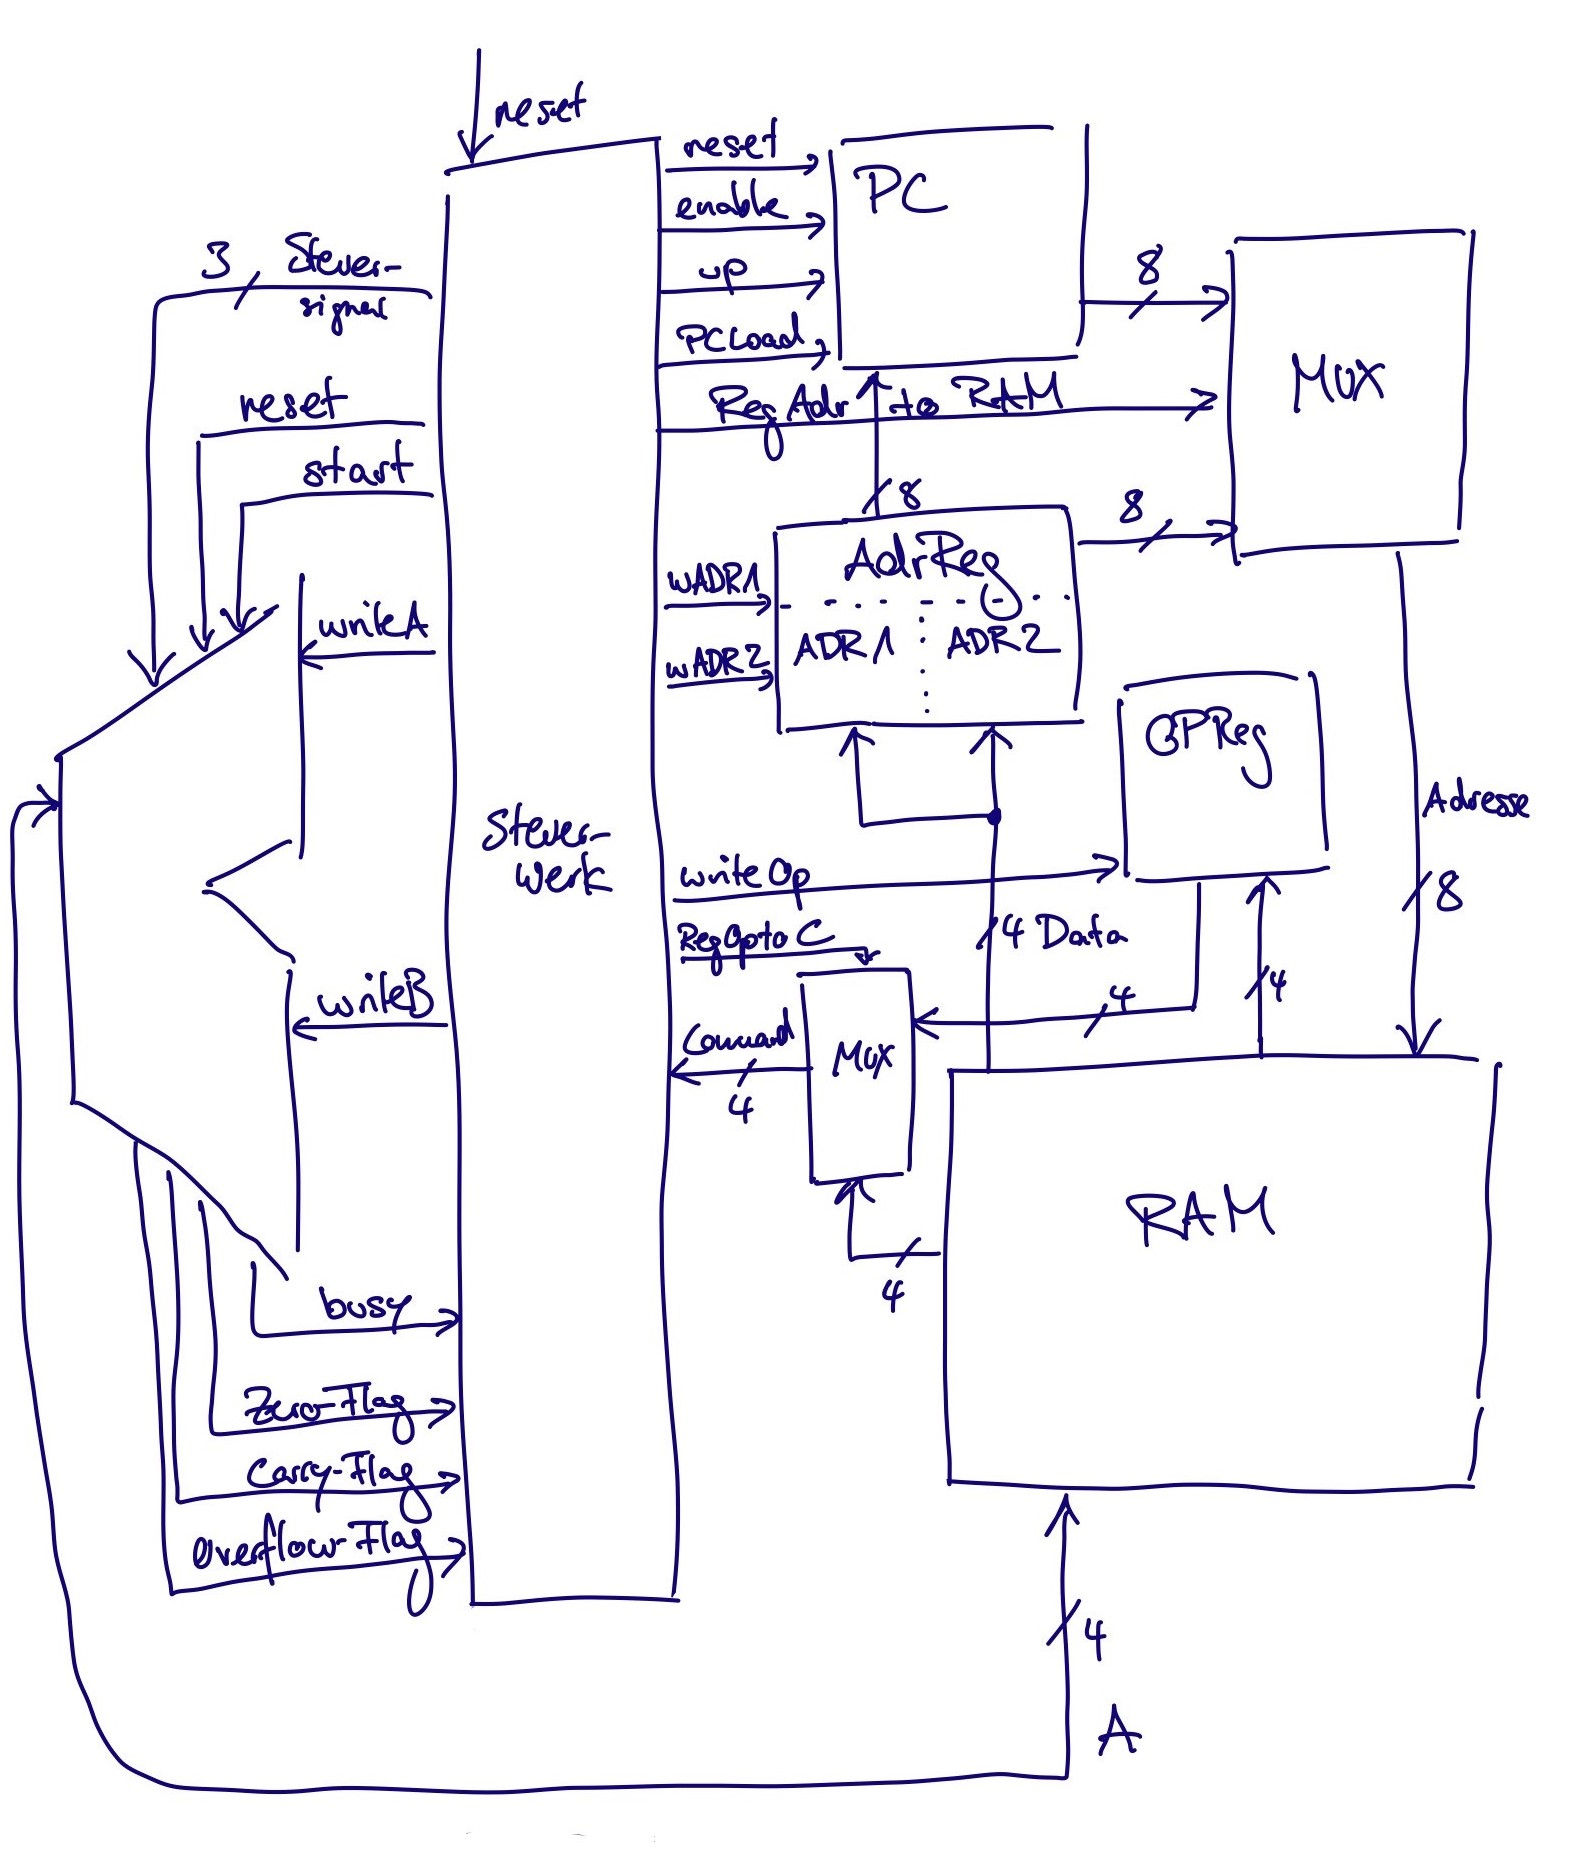
\includegraphics[scale=0.25]
  {content/figures/BSB_SW.jpg}
  \caption{First Level Blockschaltbild}
  \label{fig:blockschaltbild-first-level}
\end{figure}



\section{ALU}
Die arithmetisch-logische Einheit (ALU) ist für die Ausführung
arithmetischer sowie logischer Operationen zuständig.

\begin{table}[H]
  \begin{tabular}{|p{1.5cm}|p{2.5cm}|p{7.4592cm}|}
    \hline
    \textbf{Pins} & \textbf{Art}  & \textbf{Beschreibung}                \\
    \hline
    A3..0         & Bidirektional & Register für Operand A ($A3 = MSB$)  \\
    WriteA        & Eingang       & In A schreiben = 1 / aus A lesen = 0 \\
    \hline
    B3..0         & Bidirektional & Register für Operand B ($B3 = MSB$)  \\
    WriteB        & Eingang       & In B schreiben = 1 / aus B lesen = 0 \\
    \hline
    C2..0         & Eingang       & Register für die Operation           \\
    WriteC        & Eingang       & In C schreiben = 1                   \\
    \hline
    Start         & Eingang       & Startet die Operation (asynchron)    \\
    \hline
    Reset         & Eingang       & Beendet die Operation (synchron)     \\
    \hline
    CLK           & Eingang       & Clock                                \\
    \hline
  \end{tabular}
  \caption{Eingänge der ALU}
  \label{fig:Eingänge der ALU}
\end{table}

\begin{table}[H]
  \centering
  \begin{tabular}{|l|p{11cm}|}
    \hline
    \textbf{Pins} & \textbf{Beschreibung}                                               \\
    \hline
    BLA           &
    Gibt vorausschauend die Busy-Flag an, falls Busy mit der nächsten aktiven Flanken
    auf 0 gesetzt wird. BLA entspricht entweder Busy oder ist bereits vor der Flanke auf 0,
    nach der Busy ebenfalls auf 0 gesetzt wird.                                         \\
    \hline
    Busy          & Gibt an, ob die ALU aktuell eine Operation durchführt.
    Wenn Busy gesetzt ist, darf von außen nicht in die Register geschrieben werden.     \\
    \hline
    Carry         & Übertrag bei Addition oder Subtraktion (unsigned)                   \\
    \hline
    Overflow      & Überlauf bei Addition oder Subtraktion (signed; 2er-Kompl.)
    Das Additions- bzw. Subtraktionsergebnis ist ungültig, wenn Overflow gesetzt ist.   \\
    \hline
    Equal         & Gibt an, ob die Zahlen in Register A und B bitweise identisch sind. \\
    \hline
    Zero          & Gibt an, ob das Ergebnis der Operation an jeder Bitstelle 0 ist.    \\
    \hline
  \end{tabular}
  \caption{Ausgänge der ALU}
  \label{fig:Ausgänge der ALU}
\end{table}







\section{SWR}
\label{sec:SWR}
Das Switch Register (SWR) ermöglicht die Steuerung des Datenflusses zwischen den Registern A und B sowie
dem RAM. Es sorgt dafür, dass je nach Anforderung die entsprechenden Daten übergeben und verarbeitet werden.
Zudem übernimmt das SWR die Verteilung der Registerinhalte an die ALU zur weiteren Berechnung.

\begin{table}[H]
  \centering
  \begin{tabular}{|l|l|p{9cm}|}
    \hline
    \textbf{Signal}    & \textbf{Typ}  & \textbf{Beschreibung}                                             \\ \hline
    \textbf{WriteA}    & Eingang       & Aktiviert das Schreiben in Register A.                            \\ \hline
    \textbf{WriteRAM}  & Eingang       & Aktiviert das Schreiben von Daten in den RAM.                     \\ \hline
    \textbf{SWR}       & Eingang       & Tauscht den Inhalt von Register A und Register B.                 \\ \hline
    \textbf{A3..0}     & Bidirektional & Datenleitungen für die 4-Bit-Daten von Register A.                \\ \hline
    \textbf{B3..0}     & Bidirektional & Datenleitungen für die 4-Bit-Daten von Register B.                \\ \hline
    \textbf{RAM3..0}   & Bidirektional & Datenleitungen für die 4-Bit-Daten des RAM.                       \\ \hline
    \textbf{AluWriteA} & Ausgang       & Steuersignal zum Schreiben des Inhalts von Register A in die ALU. \\ \hline
    \textbf{AluWriteB} & Ausgang       & Steuersignal zum Schreiben des Inhalts von Register A in die ALU. \\ \hline
  \end{tabular}
  \caption{Ein- und Ausgänge des Switch Registers (SWR)}
  \label{tab:SWR}
\end{table}


\section{Programm Counter (PC)}
\label{sec:programm-counter}

Der Programm Counter (PC) zählt die auszuführenden Instruktionen und bestimmt, welche Adresse als Nächstes
verwendet wird. Der PC kann hoch- oder runterzählen und ermöglicht das Laden eines neuen Werts für
Sprungbefehle.

\begin{table}[H]
  \centering
  \begin{tabular}{|l|l|p{8cm}|}
    \hline
    \textbf{Pin}      & \textbf{Art} & \textbf{Beschreibung}                                      \\
    \hline
    \textbf{PC\_UP}   & Eingang      & Zählt den PC hoch (1) oder runter (0).                     \\ \hline
    \textbf{!PC\_LD}  & Eingang      & Lädt einen neuen Wert in den PC.                           \\ \hline
    \textbf{!PC\_EN}  & Eingang      & Aktiviert den PC für Zählvorgänge.                         \\ \hline
    \textbf{ADR7..0 } & Eingang      & Eingang für die aktuelle Adresse.                          \\ \hline
    \textbf{PC7..0 }  & Ausgang      & Gibt die aktuelle Adresse für die nächste Instruktion aus. \\ \hline
  \end{tabular} \caption{Eingänge und Ausgänge des PC}
\end{table}



\section{Adress Register (RegADR)}
\label{sec: adress-register}

Das Adressregister (RegADR) speichert die aktuelle Adresse, die entweder vom PC oder extern geladen wird,
und gibt diese an den RAM oder andere Peripherien weiter. Es sorgt für die Adressierung und Datenzugriffe.

\begin{table}[H]
  \centering
  \begin{tabular}{|l|l|p{8cm}|} \hline
    \textbf{Pin} & \textbf{Art} & \textbf{Beschreibung}                                                             \\ \hline
    WriteADR1    & Eingang      & Steuersignal zum Schreiben der oberen 4 Bits (MSB) der Adresse in Register ADR1.  \\ \hline
    WriteADR2    & Eingang      & Steuersignal zum Schreiben der unteren 4 Bits (LSB) der Adresse in Register ADR2. \\ \hline
    RAM3..0      & Eingang      & Eingang für die 4 Bits der Adressen.                                              \\ \hline
    RegADR7..0   & Ausgang      & Gibt die gespeicherte Adresse an den RAM Controller und PC weiter.                \\ \hline
  \end{tabular}
  \caption{Eingänge und Ausgänge des Adressregisters (RegADR)}
\end{table}


\section{Operations Register (OpReg)}
\label{sec: operations-register}
Das Operationsregister (OpReg) speichert die aktuelle Operation oder den Instruktionscode und gibt diesen
an die ALU weiter, um arithmetische oder logische Berechnungen durchzuführen.

\begin{table}[H]
  \centering
  \begin{tabular}{|l|l|p{8cm}|} \hline \textbf{Pin} & \textbf{Art} & \textbf{Beschreibung}                                                 \\ \hline
               RAM3..0                            & Eingang      & Lädt eine neue Operation in das Register.                             \\ \hline
               WriteOP                            & EIngang      & Steuersignal zum Schreiben der Operation in Register Op ins Register. \\ \hline
               Q3..0                              & Ausgang      & Gibt den aktuellen Instruktionscode an die ALU aus.                   \\ \hline
  \end{tabular}
  \caption{Eingänge und Ausgänge des Operationsregisters (OpReg)}
\end{table}


\section{RAM Controller}
\label{sec:ram}

Der RAM Controller steuert den Zugriff auf den RAM-Speicher. Er entscheidet, ob der RAM im Lese- oder Schreibmodus
arbeitet und welche Adresse aus dem Adressregister oder dem Program Counter verwendet wird. Der Controller
sorgt dafür, dass Daten korrekt ausgetauscht werden, ohne Konflikte zwischen Lese- und Schreiboperationen.

\begin{table}[H]
  \centering
  \begin{tabular}{|l|l|p{9cm}|}
    \hline
    \textbf{Signal}      & \textbf{Typ} & \textbf{Beschreibung}                                                          \\ \hline
    \textbf{WriteRAM}    & Eingang      & Aktiviert den Schreibvorgang im RAM.                                           \\ \hline
    \textbf{RegADRtoRAM} & Eingang      & Steuert, ob die Adresse vom Adressregister oder dem Program Counter kommt.     \\ \hline
    \textbf{RegADR7..0}  & Eingang      & 8-Bit-Adresseingänge vom Adressregister.                                       \\ \hline
    \textbf{PC7..0}      & Eingang      & 8-Bit-Adresseingänge vom Program Counter.                                      \\ \hline
    \textbf{!OE}         & Ausgang      & Ausgangsaktivierungssignal für Leseoperationen (Output Enable, aktiv niedrig). \\ \hline
    \textbf{!WE}         & Ausgang      & Aktivierungssignal für Schreiboperationen (Write Enable, aktiv niedrig).       \\ \hline
    \textbf{A7..0}       & Ausgang      & 8-Bit-Adressenleitungen zum RAM.                                               \\ \hline
  \end{tabular}
  \caption{Ein- und Ausgänge des RAM Controllers}
  \label{tab:RAM_Controller}
\end{table}











